\section{Optimizations}\label{s:search}
This section describes our system optimizations.

\begin{figure}[t]
    \centering
    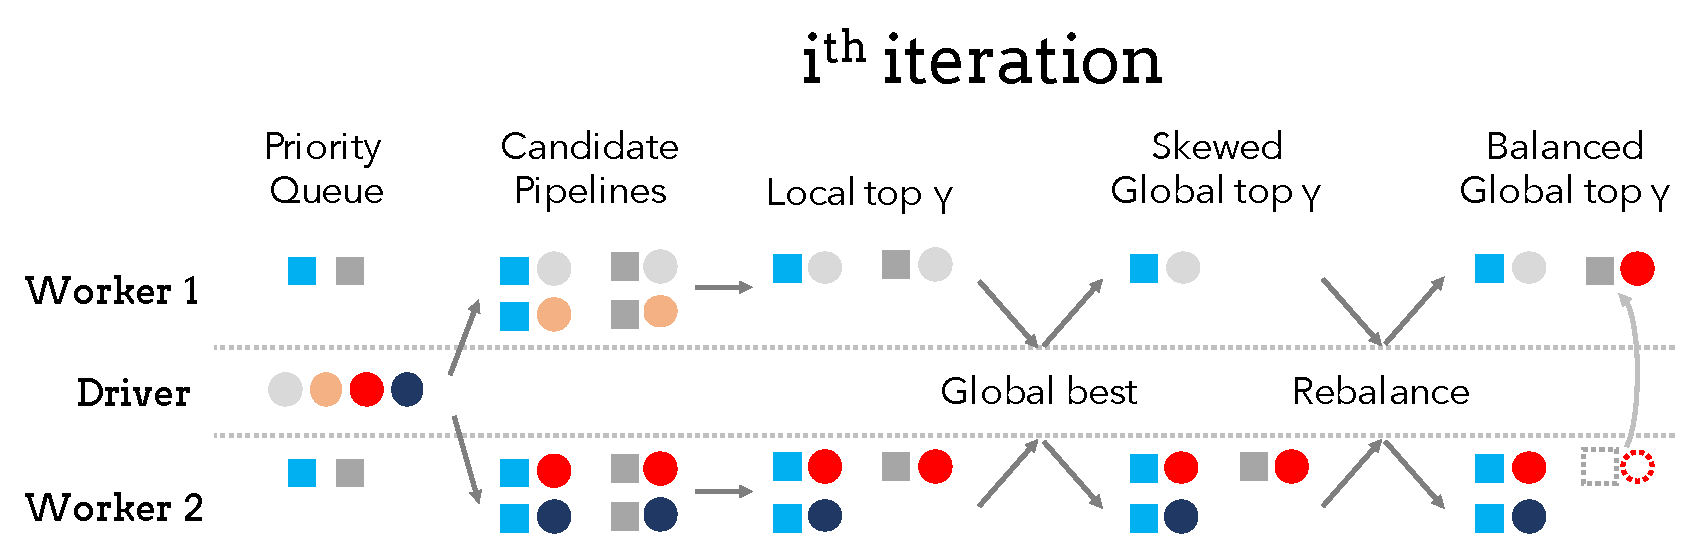
\includegraphics[width=\columnwidth]{figures/distributed.pdf}
    \caption{In each iteration, each worker starts with a subset of the priority queue (boxes).  The driver sends a subset of data transformations from $\Sigma$ (circles) to generate candidate pipelines (box-circles).  A series of synchronization points identify the globally top $\gamma$ candidates and redistributes them across the workers.   \label{fig:algo}}
\end{figure}


{
\begin{algorithm}[t]
\KwData{Q, S}

 Pruned = $\{\}$  //empty priority queue

 \For{$s \in S$ }{
 
    $\bar{s}$ = $s$
    
    \For{$s' \in S$ }{
        
        $m$ :=  $s' \circ \bar{s}$
        
        $\bar{s}_{pred}$ := $\cup_{c\in \bar{s}} c.pred$
        
        $s_{pred}'$ := $\cup_{c\in s'} c.pred$
        
        
        \If{$\bar{s}_{pred} \cap s_{pred}' = \emptyset$ and $Q(\bar{s}) < Q(m)$}{
        
           $\bar{s} = m$
        }
        
    }
    
    Pruned.push($\bar{s}$)
        
}


\Return Pruned
\caption{Pruning Disjoint Paths}
\label{alg:pruning}
\end{algorithm}
}


\subsection{Parameter Space Sampler}
By default, users simply specify the domain of an operator parameter as a list of values, and \sys uniformly samples from the domain.  In addition, users can specify two types of parameters, for which \sys can apply search optimizations:

\begin{itemize}[leftmargin=*,topsep=.3em,itemsep=-.2em,partopsep=-.5em]
  \item \stitle{Attribute Name Parameters} If the parameter represents an attribute in the database, then \sys can infer the domain of allowable values.   For example, a numerical outlier detection algorithm might apply to a single attribute or a subset of attributes. \sys can also prune the paramater space by pruning attribute names that are irrelevant to the quality function.  

  \item \stitle{Threshold Parameters} Numeric parameters are often used as thresholds, inference parameters, or confidence bounds.  For these, users specify the most and least restrictive ends of the value domain, and \sys will sweep the space from most to least restrictive.   For instance, \texttt{ispell} only uses the dictionary if the attribute value is within \texttt{rec} characters of the dictionary word.  Thus, \sys will initially sample $\texttt{rec}=0$ and gradually relax the threshold.   
\end{itemize}

%which have the property that if the quality function    Another broad class of parameters in data cleaning methods are numerical parameters like thresholds and inference parameters. For these parameters, the user specifies a range (or a multi-dimensional grid). Often times, these parameters correspond to confidence metrics. In the example with the \texttt{City} table, the \texttt{ispell} method has a acceptance threshold for spell-checking. In these cases, we recommend that this search space is ordered fine-to-coarse. Where the most restrictive threshold is evaluated first towards increasingly less restrictive thresholds. 


\subsection{Incremental Quality Evaluation}\label{s:qualityivm}

Most cleaning operators modify significantly fewer records than the entire dataset.  Since quality functions are simply aggregation queries, \sys can incrementally evaluate the quality function over the fixed records rather than the full dataset.  
This is exactly the process of incremental view maintenance, and we use standard techniques to incrementally compute quality functions that \ewu{HAVE X and Y properties}.  

Suppose we have relation $R$, quality function $q$, and a set of conditional assignment expressions $C$.  When possible, \sys computes $q(R)$ once and then for each of the expressions $c \in C$ compute a delta such $q(c(R)) = q(R) + \delta_c(q(R))$.
For many types of quality functions such incremental computation can be automatically synthesized and can greatly save on computation time.

Let us consider a concrete example with the quality function $q_1$, a functional dependency checker, from the previous section.
$R'$ is the resulting relation after applying \texttt{c} to all of the records.
Let $r_{pred}$ be the set of records that satisfy the predicate of the conditional assignment expression and $r_{pred}'$ be the resulting transformed records.
$q_1$ can be expressed in relational algebra in the following way:
\[
q_1(R') = \textsf{count}( R' \bowtie R' )
\]
$R'$ can be described in terms of $R$:
\[
R' = R - r_{pred} + r_{pred}' 
\]
leading to the following expression:
\[
q_1(R') = \red{q_1(R)} - \textsf{count}( r_{pred} \bowtie R )  + \textsf{count}( r'_{pred} \bowtie R )
\]
If we used a hash join to evaluate this quality function, the cost of incrementally maintaining is roughly linear in the size of the number records changed rather than the size of the relation.

% The consequence is that evaluating changes in quality can be very efficient for a large class of data cleaning problems.  The architecture of \sys is designed to exploit this property.  We assume conditional assignment generation to be expensive but quality evaluation to be fast.  An architecture that runs the entire pipeline before seeing the resultant quality is wasteful.






\subsection{Pipeline Merging}
In general, conditional assignments are not commutative, meaning that $c_i\circ c_j \ne c_j\circ c_i$.  Thus, each possible ordering must be explored sequentially, which leads to an exponential search-space growth.  For instance, with $k$ conditional assignments, there are $\sum_{n\le k} n!$ possible orderings up to length $k$.  However, if $c_i$ and $c_j$'s predicates are non-overlapping, then their operations are commutative ($c_i\circ c_j = c_j\circ c_i$) and reduces the search space to $2^k$.  Based on this observation, we use a heuristic to opportunistically merge candidate pipelines if their predicates are disjoint and the resulting pipeline increases the quality function.  Specifically, let predicate $s_{pred}$ be the union of all of the predicates of each conditional assignment in $s$.  If two candidate pipelines $\bar{s},s'$ have disjoin predicates $\bar{s}_{pred}$ and $s'_{pred}$, then we replace both candidates if their composition has a higher quality.  \Cref{alg:main} describes the algorithm.


\subsection{Parallelization} 
Even with incremental evaluation, composing and evaluating $Q(s'(R))$ is the single most expensive search operation.  Thus, we parallelize across candidate pipelines and across data partitions.  Our implementation uses Ray~\cite{ray} to schedule and parallelize the tasks over multiple CPUs and machines.

\stitle{Search Parallelism}
Conceptually, we execute all expansions for a given plan $s$ in parallel.  We materialize the incremental deltas in memory, and evaluate the quality of each $s' = c\circ s$ in parallel using a thread pool.  Each thread drops a given $s'$ if its quality is lower than $\gamma\times$ the maximum quality from the previous \texttt{WHILE} iteration or the local thread.  At the end of the \texttt{WHILE} iteration, the threads synchronize to compute the highest quality, and flush the remaining candidates using the up-to-date quality value.


The implementation of this conceptual parallelization is a little bit more complex. 
Each worker is given a subset of candidate pipelines to locally evaluate and prune, and the main challenge is to reduce task skew through periodic rebalancing.  We use a worker-driver model with $j$ workers (\Cref{fig:algo}).

Let $S^{next} = S\times P$ be the set of candidate pipelines (e.g., 
\includegraphics[height=8pt]{figures/program.pdf}) to evaluate in the current iteration of the search algorithm. For instance, $S=\{NOOP\}$ in the first iteration, so the candidates are the set of individual data transformations $P$.   The driver assigns the input relation $R$ and $\frac{1}{j}$ of $P^{next}$ to each worker.  In the figure, the driver assigns a subset of $\Sigma$ to each worker.  Each worker evaluates and computes the top-$\gamma$ candidates based on the best worker-local quality.   The worker runs and caches the parents of its assigned candidate pipelines (
\includegraphics[height=8pt]{figures/sq-blue.pdf}, 
\includegraphics[height=8pt]{figures/sq-grey.pdf}) to incrementally compute the quality function.
  
Note that the worker-local top-$\gamma$ candidates are a superset of the top-$\gamma$ global candidates because the best local quality is $\le$ the global best.   Thus the workers synchronize with the driver to identify the global best candidate and further prune each worker's top candidates.  At this point, all candidate pipelines are within $\gamma$ of the globally best candidate, but their distribution across the workers can be highly skewed.  \sys performs a final rebalancing step, where each worker sends the number of un-pruned candidates to the driver.  Workers with more than $\frac{1}{j}$ of the total number redistribute the extras to workers with too few candidates.  When redistributing, workers communicate directly and do not involve the driver (e.g., Worker 2 sends 
\includegraphics[height=8pt]{figures/program-greyred.pdf} to Worker 1).   If the total number is $<k$, then candidates are randomly chosen to be replicated.  Only the pipelines and their qualities are sent; the pipeline results are re-computed by the receiving worker.  This ensures that the priority queue in the next iteration is evenly distributed across all workers.

\stitle{Data Parallelism}
Many large datasets are naturally partitioned, e.g., by timestamp or region. 
The idea is to partition the dataset in such a way that errors are local to a small number of records.
This means that a fix for a given record does not affect the other records outside of the partition.
There is a relationship between partitioning and the quality functions defined.
For example, quality functions derived from functional dependencies can define blocks by examining the violating tuples linked through the dependency.  Similarly, users can define custom partitioning functions.  In our current implementation, we partition the input relation by row by user-specified blocking rules.

